\documentclass{standalone}
% 

% \pgfmathdeclarefunction{gauss}{2}{%
%   \pgfmathparse{1/(#2*sqrt(2*pi))*exp(-((x-#1)^2)/(2*#2^2))}%
% }
\usepackage{tkz-euclide}
\usetkzobj{all}
\renewcommand{\familydefault}{\sfdefault}
\usepackage{calc,tikz}
\usetikzlibrary{calc}
\usepackage{pgfplots}
\begin{document}
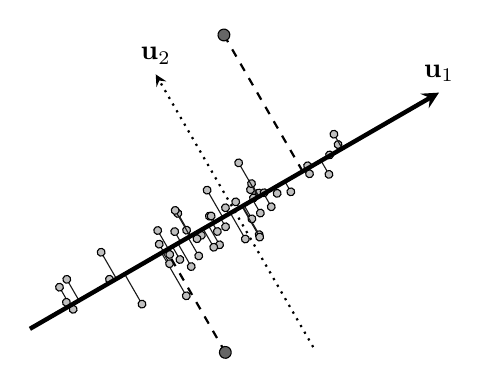
\begin{tikzpicture}[>=stealth]
    \def\normaltwo{\x,{4*1/exp(((\x-0)^2)/2)}}
    % \node [scale = 2] at (6.5, 3.3) {PCA procedure};
   
    %%%%%%%%%% block 6 %%%%%%%%%%%%%%%%%%%
    % \node [scale = 1.25, text width = 4cm] at (0, -4) {7. Obtain projected points in low dimension.};
    \begin{scope}[xshift = 0cm, yshift = -7cm, rotate = 30]
        % \draw [rounded corners = 1pt, thick] (-2.7, -3) rectangle (3.3, 3.82);
    \begin{scope}[rotate = 0, xshift = .5]
        \tkzDefPoint(180:3){A}
        \tkzDefPoint(0:4){B}
        % \draw [<-, very thick, dashed] (A)  --  (B);
        % \draw [<-, very thick, dashed] ($(0,0) + (150:2)$)  --  ($(0,0) + (-30:2)$);
       
        \draw[->, dotted, thick, black] (0, -2)  --  ($ (0, 2)$) node[above] {$\mathbf{u}_2$};
        % \draw[->, ultra thick, red] (0, 0)  --  ($(0,0) + (150:2)$) node[right] {$\mathbf{u}_2$};
        % \draw[->, thick] (-1,0)  --  (2,0) node[right] {$\mathbf{e}_1$};
        % \draw[->, thick] (-0,-2)  --  (-0,2) node[right] {$\mathbf{e}_2$};


        \begin{scope}[rotate = 0]
            \foreach \x/\y/\z in {-0.32/-0.12/0, -0.06/-0.38/1, 1.27/-0.20/2, -0.31/0.10/3, 0.58/-0.08/4, -0.79/0.15/5, 0.31/0.13/6, -0.99/-0.07/7, 0.38/0.04/8, 0.12/-0.42/9, 0.07/0.09/10, 1.09/0.03/11, 0.29/0.02/12, -0.17/0.40/13, 0.36/0.19/14, 0.14/-0.20/15, -0.38/-0.28/16, -1.61/-0.44/17, -0.52/-0.06/18, 0.43/-0.19/19, 1.56/0.07/20, 1.58/0.21/21, -0.83/-0.34/22, 0.27/-0.19/23, -0.29/0.09/24, -2.41/0.27/25, -2.28/0.31/26, -0.20/-0.12/27, -0.64/0.33/28, 1.06/-0.07/29, -0.91/-0.19/30, -0.65/0.09/31, -0.68/-0.27/32, -1.07/-0.63/33, -2.43/0.06/34, -0.97/0.27/35, 1.40/0.01/36, -0.46/-0.27/37, 0.11/-0.45/38, -0.08/0.09/39, -1.81/0.04/40, 0.44/0.01/41, -2.40/-0.06/42, 0.74/-0.15/43, -1.05/-0.17/44, -0.59/-0.07/45, -0.65/0.38/46, 0.35/0.50/47, -1.73/0.39/48, -1.04/0.11/49 } {

                % \tkzDefPoint(\x, \y){x\z}
                \draw [black!90] (\x, \y)  --  (\x, 0);
                \draw [fill = gray!50] (\x, \y) circle (.5mm); 
                % \tkzDefPointBy[projection=onto B -- A](x\z)
                % \tkzGetPoint{H\z}
                % \tkzDrawLines[add = 0 and 0, thick, green](x\z,H\z)
                % \draw [fill = red!90] (H\z) circle (1mm); 

                }

            \draw [black, dashed, thick] (1, 2)  --  (1, 0);
            \draw [fill = gray!80!black] (1, 2) circle (.75mm);
            \draw [black, dashed, thick] (-1, -1.5)  --  (-1, 0);
            \draw [fill = gray!80!black] (-1, -1.5) circle (.75mm);
        \end{scope}
         \draw[->, ultra thick, black] (-3, 0)  --  ($ (3, 0)$) node[above] {$\mathbf{u}_1$};
        % \node [scale = 1.5, red] at (1, -1.5) {$\mathbf{Z}$};
    \end{scope}
    \end{scope}


    

\end{tikzpicture}
\end{document}